\documentclass[border={0.1cm 0.1cm 0.1cm 0.1cm}]{standalone}  %E,S,W,N

\usepackage{amssymb}
\usepackage{amsmath}
\usepackage{tikz}
\usetikzlibrary{decorations.pathreplacing}	%for brackets

\begin{document}
	
	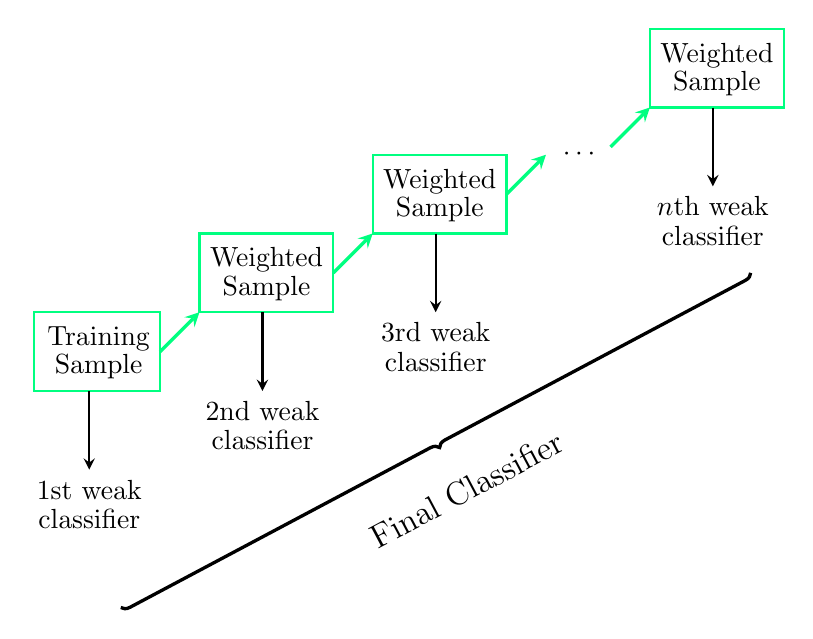
\begin{tikzpicture}	
	\def\x{0} \def\y{0}
	\draw[green!50!cyan,fill=white,thick] (\x-1.1,\y-0.5) rectangle (\x+0.5,\y+0.5) node[below left,black,align=center,yshift=-0.5mm] {Training \\[-0.6mm] Sample};
	
	\foreach \i in {1,2,3.6}{
		\draw[green!50!cyan,fill=white,thick] (2.2*\i-1.2,\i-0.5) rectangle (2.2*\i+0.5,\i+0.5) node[below left,black,align=center,yshift=-0.5mm] {Weighted\\[-0.6mm] Sample};
	}
	
	%DIAGONAL ARROWS
	\draw[very thick,->,>=stealth,green!50!cyan] (2.2*0+0.5,0)--(2.2*1-1.2,1-0.5);
	\draw[very thick,->,>=stealth,green!50!cyan] (2.2*1+0.5,1)--(2.2*2-1.2,2-0.5);
	\draw[very thick,->,>=stealth,green!50!cyan] (2.2*2+0.5,2)--(2.2*3-1.2,3-0.5);
	\node at (2.2*2.5+0.35,2.5) {$\cdots$};
	\draw[very thick,->,>=stealth,green!50!cyan] (2.2*2.6+0.5,2.6)--(2.2*3.6-1.2,3.6-0.5);
	
	%WEAK CLASSIFIER ARROWS
	\draw[->,>=stealth,thick] (2.2*0-0.4,0-0.5)--++(0,-1) node[below,align=center,black] {1st weak \\[-0.5mm] classifier};
	\draw[->,>=stealth,thick] (2.2*1-0.4,1-0.5)--++(0,-1) node[below,align=center,black] {2nd weak \\[-0.5mm] classifier};
	\draw[->,>=stealth,thick] (2.2*2-0.4,2-0.5)--++(0,-1) node[below,align=center,black] {3rd weak \\[-0.5mm] classifier};
	\draw[->,>=stealth,thick] (2.2*3.6-0.4,3.6-0.5)--++(0,-1) node[below,align=center,black] {$n$th weak \\[-0.5mm] classifier};
	
	%BRACKETS
	\draw[decorate,decoration={brace,amplitude=3pt},very thick] (8,1)--(0,-3.25);
	\node[right,align=left] at (3,-1.75) {\rotatebox{28}{\large Final Classifier}};
	\end{tikzpicture}
	
\end{document}